\chapter{Search problems}



\section{Search strategies}
\begin{description}
    \item[Solution space] \marginnote{Solution space}
        Set of all the possible sequences of actions an agent may apply.
        Some of these lead to a solution.
    
    \item[Search algorithm] \marginnote{Search algorithm}
        Takes a problem as input and returns a sequence of actions that solves the problem (if exists).
\end{description}


\subsection{Search tree}
\begin{description}
    \item[Expansion] \marginnote{Expansion}
        Starting from a state, apply a successor function and generate a new state.

    \item[Search strategy] \marginnote{Search strategy}
        Choose which state to expand. 
        Usually is implemented using a fringe that decides which is the next node to expand.

    \item[Search tree] \marginnote{Search tree}
        Tree structure to represent the expansion of all states starting from a root 
        (i.e. the representation of the solution space).

        Nodes are states and branches are actions.
        A leaf can be a state to expand, a solution or a dead-end.
        \Cref{alg:search_tree_search} describes a generic tree search algorithm.

        \begin{figure}[h]
            \centering
            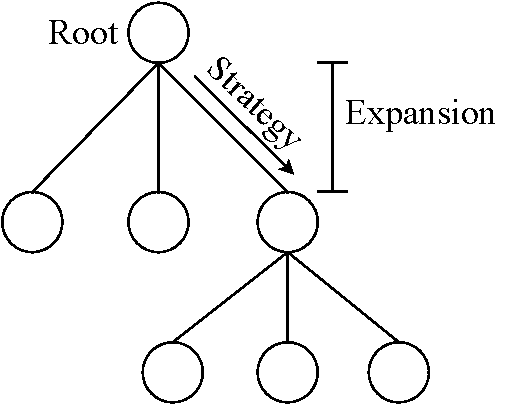
\includegraphics[width=0.25\textwidth]{img/_search_tree.pdf}
            \caption{Search tree}
        \end{figure}

        Each node contains:
        \begin{itemize}
            \item The state
            \item The parent node
            \item The action that led to this node
            \item The depth of the node
            \item The cost of the path from the root to this node
        \end{itemize}
\end{description}

\begin{algorithm}
\caption{Tree search algorithm} \label{alg:search_tree_search}
\begin{lstlisting}
def treeSearch(problem, fringe):
    fringe.push(problem.initial_state)
    # Get a node in the fringe and expand it if it is not a solution
    while fringe.notEmpty():
        node = fringe.pop()
        if problem.isGoal(node.state):
            return node.solution
        fringe.pushAll(expand(node, problem))
    return FAILURE

def expand(node, problem):
    successors = set()
    # List all neighboring nodes
    for action, result in problem.successor(node.state):
        s = new Node(
            parent=node, action=action, state=result, depth=node.dept+1,
            cost=node.cost + problem.pathCost(node, s, action)
        )
        successors.add(s)
    return successors
\end{lstlisting}
\end{algorithm}


\subsection{Strategies}
\begin{description}
    \item[Non-informed strategy] \marginnote{Non-informed strategy}
        Domain knowledge not available. Usually does an exhaustive search.

    \item[Informed strategy] \marginnote{Informed strategy}
        Use domain knowledge by using heuristics.
\end{description}


\subsection{Evaluation}
\begin{description}
    \item[Completeness] \marginnote{Completeness}
        if the strategy is guaranteed to find a solution (when exists).

    \item[Time complexity] \marginnote{Time complexity}
        time needed to complete the search.

    \item[Space complexity] \marginnote{Space complexity}
        memory needed to complete the search.

    \item[Optimality] \marginnote{Optimality}
        if the strategy finds the best solution (when more solutions are possible).
\end{description}



\section{Non-informed search}

\subsection{Breadth-first search (BFS)}
\marginnote{Breadth-first search}
Always expands the less deep node. The fringe is implemented as a queue (FIFO).

\begin{center}
    \def\arraystretch{1.2}
    \begin{tabular}{c | m{10cm}}
        \hline
        \textbf{Completeness} & Yes \\
        \hline
        \textbf{Optimality} & Only if cost is uniform (i.e. all edges have same cost) \\
        \hline
        \textbf{\makecell{Time and space\\complexity}}
            & $O(b^d)$, where the depth is $d$ and the branching factor is $b$ (i.e. each non-leaf node has $b$ children) \\
        \hline
    \end{tabular}
\end{center}

The exponential space complexity makes BFS impractical for large problems.

\begin{figure}[h]
    \centering
    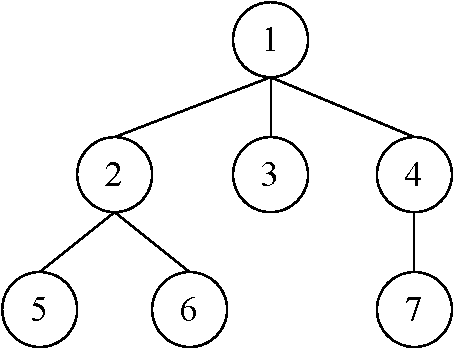
\includegraphics[width=0.40\textwidth]{img/_bfs.pdf}
    \caption{BFS visit order}
\end{figure}


\subsection{Uniform-cost search}
\marginnote{Uniform-cost search}
Same as BFS, but always expands the node with the lowest cumulative cost. 

\begin{center}
    \def\arraystretch{1.2}
    \begin{tabular}{c | m{10cm}}
        \hline
        \textbf{Completeness} & Yes \\
        \hline
        \textbf{Optimality} & Yes \\
        \hline
        \textbf{\makecell{Time and space\\complexity}}
            & $O(b^d)$, with depth $d$ and branching factor $b$ \\
        \hline
    \end{tabular}
\end{center}

\begin{figure}[h]
    \centering
    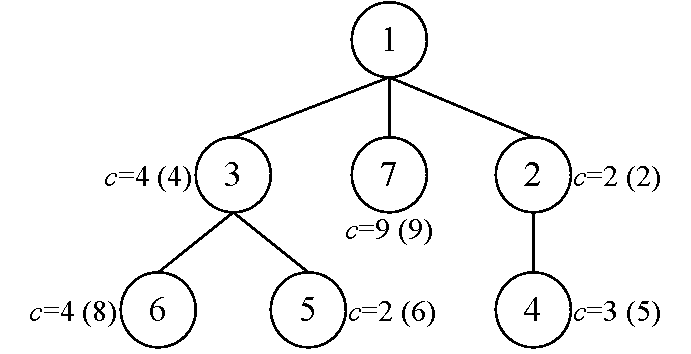
\includegraphics[width=0.60\textwidth]{img/_ucs.pdf}
    \caption{Uniform-cost search visit order. $(n)$ is the cumulative cost}
\end{figure}


\subsection{Depth-first search}
\marginnote{Depth-first search}
Always expands the deepest node. The fringe is implemented as a stack (LIFO).

\begin{center}
    \def\arraystretch{1.2}
    \begin{tabular}{c | m{10cm}}
        \hline
        \textbf{Completeness} & No \\
        \hline
        \textbf{Optimality} & No \\
        \hline
        \textbf{Time complexity}
            & $O(b^d)$, with depth $d$ and branching factor $b$ \\
        \hline
        \textbf{Space complexity}
            & $O(b \cdot d)$, with depth $d$ and branching factor $b$ \\
        \hline
    \end{tabular}
\end{center}

\begin{figure}[h]
    \centering
    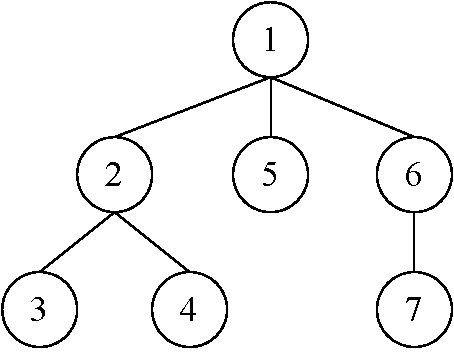
\includegraphics[width=0.40\textwidth]{img/_dfs.pdf}
    \caption{DFS visit order}
\end{figure}